\documentclass{report}
\usepackage{graphicx}
\usepackage{pgfplots}
\usepackage{booktabs}
\usepackage{amsmath,amssymb}
\pgfplotsset{compat=1.18}

\author{Trinh Thanh Vinh}
\title{Labwork 3: CUDA}

\begin{document}
\maketitle

\section{Introduction}
The objective for this labwork is to improve the RGB-to-grayscale CUDA program from Labwork 3 by replacing its 1D thread organization with a 2D grid of 2D blocks. Multiple 2D block sizes were tested, the execution times were measured, and the results were compared with the earlier 1D implementation.

\section{Implementation}
This labwork was conducted on the same hardware setting mentioned in the previous report.

In Labwork 3, the image was flattened into a list of pixels. A thread used a single global index to select one pixel. In Labwork 4, the image remains in its original $H\times W\times 3$ representation. The kernel obtains its column and row indices independently. For each valid coordinate, the thread reads the red, green, and blue values, computes their arithmetic mean, and writes that grayscale value to all three output channels.

Before a thread reads or writes a pixel, it checks that $x < W$ and $y < H$. This check stops extra threads from using memory outside the image. Extra threads can appear when the image width or height is not an exact multiple of the block size. For this reason, the program rounds up when it calculates the grid size:
\[
  G_x = \left\lceil\frac{W}{B_x}\right\rceil, \qquad
  G_y = \left\lceil\frac{H}{B_y}\right\rceil.
\]

This grid covers the complete image. It also gives a direct connection between the position of a thread and the position of a pixel. Threads next to each other in the $x$ direction read pixels next to each other. This pattern helps the GPU access global memory efficiently.

Before starting the timing, the kernel was run once as a warm-up. After that, the program runs the kernel five times and waits for the GPU to finish. It reports the average running time. The tested 2D block sizes were $8\times8$, $16\times16$, and $32\times32$. They contain 64, 256, and 1024 threads per block, respectively.

\section{Results}
As shown in Table~\ref{tab:results}, the execution times vary across different block configurations. 

\begin{table}[ht]
  \centering
  \caption{Timing result between 1D and 2D implementation}
  \label{tab:results}
  \begin{tabular}{ccccc}
    \toprule
    2D block & Threads/block & 1D time ($\mu$s) & 2D time ($\mu$s) & Speedup \\
    \midrule
    $8\times8$   & 64   & 161.48 & 191.16 & $0.845\times$ \\
    $16\times16$ & 256  & 161.32 & 157.24 & $1.026\times$ \\
    $32\times32$ & 1024 & 158.74 & 170.22 & $0.933\times$ \\
    \bottomrule
  \end{tabular}
\end{table}

Figure~\ref{fig:speedup} depicts the relationship between the 2D block size and its speedup over the corresponding 1D configuration. A bar taller than 1 means that the 2D configuration is faster than the matched 1D configuration. A bar shorter than 1 means that the 2D configuration is slower.

\begin{figure}[ht]
  \centering
  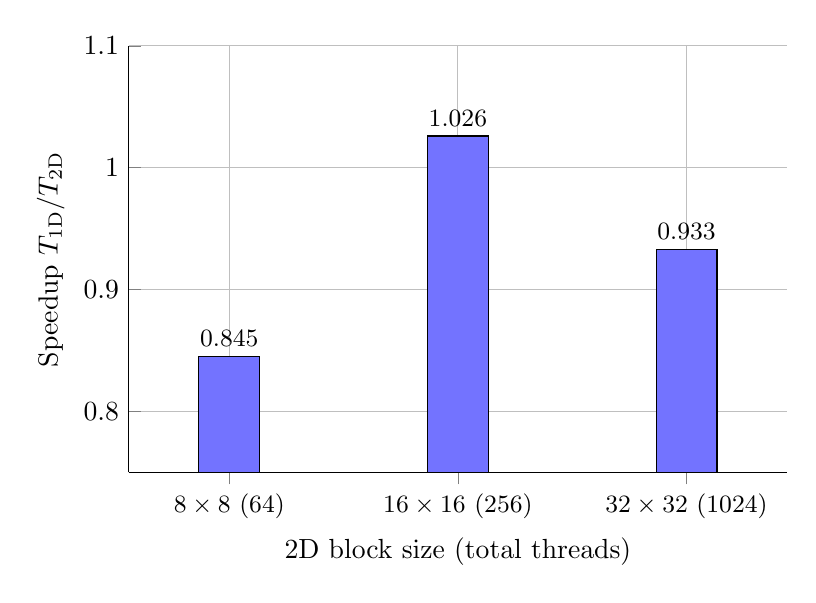
\begin{tikzpicture}
    \begin{axis}[
      width=0.82\textwidth,
      height=7cm,
      ybar,
      bar width=22pt,
      ymin=0.75,
      ymax=1.10,
      ylabel={Speedup $T_{\mathrm{1D}}/T_{\mathrm{2D}}$},
      xlabel={2D block size (total threads)},
      symbolic x coords={$8\times8$ (64),$16\times16$ (256),$32\times32$ (1024)},
      xtick=data,
      x tick label style={font=\small},
      nodes near coords={\pgfmathprintnumber[fixed,precision=3]{\pgfplotspointmeta}},
      nodes near coords style={font=\small},
      grid=major,
      axis lines*=left,
      enlarge x limits=0.22
    ]
      \addplot[fill=blue!55] coordinates {
        ($8\times8$ (64),0.845)
        ($16\times16$ (256),1.026)
        ($32\times32$ (1024),0.933)
      };
    \end{axis}
  \end{tikzpicture}
  \caption{Speedup of each 2D configuration over the 1D configuration with the same number of threads per block.}
  \label{fig:speedup}
\end{figure}

The fastest 2D block size was $16\times16$, with a kernel time of $157.24\,\mu$s. It was about $2.6\%$ faster than the 1D version with 256 threads per block. The $8\times8$ block was about $15.5\%$ slower than the 1D version with 64 threads. The $32\times32$ block was about $6.7\%$ slower than the 1D version with 1024 threads. The best 2D time was $157.24\,\mu$s, and the best 1D time was $158.74\,\mu$s. Therefore, the best 2D result was about $0.95\%$ faster.

\section{Exercises}
\subsection{Exercise 1}
The GPU in this exercise allows a maximum of 512 threads per block, 1024 threads per SM, eight blocks per SM, and 32 threads per warp.
For an $8\times8$ block, there are
\[
 8\times8=64\text{ threads per block}.
\]
The thread limit alone would allow $1024/64=16$ blocks. However, the SM can only hold eight blocks. Therefore, the SM can use
\[
 8\text{ blocks}\times64\text{ threads}=512\text{ active threads}.
\]
This uses only half of the 1024 available thread positions.
For a $16\times16$ block, there are
\[
 16\times16=256\text{ threads per block}.
\]
The SM can hold $1024/256=4$ of these blocks. Four is below the limit of eight blocks, so four blocks can run at the same time. They use
\[
 4\text{ blocks}\times256\text{ threads}=1024\text{ active threads}.
\]
This uses all available thread positions on the SM.
For a $32\times32$ block, there are
\[
 32\times32=1024\text{ threads per block}.
\]
This is higher than the limit of 512 threads per block. Therefore, this block size is not valid on the GPU described in the exercise.

The best choice is therefore $16\times16$. It is valid, uses all 1024 thread positions on the SM, and has $256/32=8$ full warps in each block.

\subsection{Exercise 2}
The SM has two limits. First, it can run no more than four blocks at the same time. Second, all active blocks together can contain no more than 1536 threads. Both limits must be followed. For each block size, we first calculate how many blocks can fit within 1536 threads. If this answer is greater than four, only four blocks can run. In other words:
\[
 \text{active blocks}
 =\min\left(4,\left\lfloor
 \frac{1536}{\text{threads per block}}
 \right\rfloor\right).
\]

For 128 threads per block, the thread limit would allow $\lfloor1536/128\rfloor=12$ blocks. The four-block limit reduces this to four blocks, so there are $4\times128=512$ active threads.

For 256 threads per block, the thread limit would allow six blocks. Again, only four blocks are allowed, so there are $4\times256=1024$ active threads.

For 512 threads per block, exactly three blocks fit because $1536/512=3$. This gives $3\times512=1536$ active threads.

For 1024 threads per block, only one block fits. Two blocks would need 2048 threads, which is higher than the limit. Therefore, this choice gives 1024 active threads.

Therefore, 512 threads per block is the best choice when only the limits given in the exercise are considered. It allows three blocks and uses all 1536 thread positions on the SM.

\subsection{Exercise 3}
The vector has 2000 elements, and each block contains 512 threads. One thread works on one vector element. To find the number of blocks, we divide the number of elements by the number of threads in one block:
\[
 \frac{2000}{512}=3.90625.
\]
A CUDA grid cannot contain part of a block, so the result must be rounded up to the next whole number. Therefore, the required number of blocks is
\[
 \left\lceil\frac{2000}{512}\right\rceil=4.
\]
Four blocks create
\[
 4\times512=2048\text{ threads}.
\]
Thus, the answer is 2048 threads in the grid. Of these, 2000 threads process vector elements and 48 threads are extra.
\end{document}